%%% lorem.tex --- 
%% 
%% Filename: lorem.tex
%% Description: 
%% Author: Ola Leifler
%% Maintainer: 
%% Created: Wed Nov 10 09:59:23 2010 (CET)
%% Version: $Id$
%% Version: 
%% Last-Updated: Tue Oct  4 11:58:17 2016 (+0200)
%%           By: Ola Leifler
%%     Update #: 7
%% URL: 
%% Keywords: 
%% Compatibility: 
%% 
%%%%%%%%%%%%%%%%%%%%%%%%%%%%%%%%%%%%%%%%%%%%%%%%%%%%%%%%%%%%%%%%%%%%%%
%% 
%%% Commentary: 
%% 
%% 
%% 
%%%%%%%%%%%%%%%%%%%%%%%%%%%%%%%%%%%%%%%%%%%%%%%%%%%%%%%%%%%%%%%%%%%%%%
%% 
%%% Change log:
%% 
%% 
%% RCS $Log$
%%%%%%%%%%%%%%%%%%%%%%%%%%%%%%%%%%%%%%%%%%%%%%%%%%%%%%%%%%%%%%%%%%%%%%
%% 
%%% Code:

\chapter{Teori}
\label{cha:theory}

Nedan presenteras hur Entropi-estimering, Huffman-kodning och LZW-kodning fungerar.

\subsection{Entropi-estimering}
Det går att mäta hur bra komprimerad en sekvens är, detta gör man genom mäta takten på koden. Takten på koden ges av \cite{nautsch2018}.

\bigskip
\noindent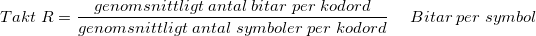
\includegraphics{TaktFormula.png}

\bigskip 
\noindent Det ger alltså ett tal som säger i snitt hur många bitar vi har kodat varje symbol med.

Entropin för en källa är en teoretisk lägre gräns för hur många bitar vi behöver för att koda varje symbol. Takten kan alltså inte vara under denna gräns. Entropin av en källa ges av \cite{nautsch2018}.

\bigskip 
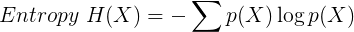
\includegraphics{EntropyFormula.png}

\bigskip 
\noindent Där p(X) är sannolikheten för given symbol och log är bas 2 logaritm. Vi summerar över alla symboler i källan.


\subsection{Huffman-kodning}
Huffman-kodning är en metod för att komprimera filer till ett mindre format. Metoden utvecklades av  den dåvarande studenten David A. Huffman år 1952. Idén med metoden är att tilldela varje symbol som ska kodas en sekvens av olika bitar, 0 eller 1, exempel:

\bigskip
\noindent Symbol A kodas till 10101010

\noindent Symbol B kodas till 1000000

\noindent Symbol C kodas till 11111111

\bigskip
\noindent I metoden kommer de symboler som förekommer flest gånger i källan, det vill säga den symbol som har högst sannolikhet, att tilldelas minst antal bitar. Det betyder att de symboler som förekommer minst gånger i källan kommer tilldelas mest antal bitar. Exempel kan symbolen D kodas med bitarna 10 och symbolen E kodas med bitarna 1001010101. Det betyder att symbolen D förekommer oftare i sekvensen än symbolen E. Alltså kommer sekvensen att komprimeras på bästa möjliga vis.  Redan här inses att med Huffman-kodning behövs information om hur källan ser ut. Det vill säga, man behöver veta sannolikheterna för de olika symbolerna i källan. Nedan beskrivs mer ingående hur komprimering och avkomprimering fungerar i Huffman-kodning \cite{huffmancoding2018}.
	\subsubsection{Komprimering}
	Att komprimera en källa med Huffman-kodning förutsätter att det finns en given sannolikhetstabell för källan. Det finns alltså en lista som mappar en symbol mot dess sannolikhet, vi kallar här varje symbol och dess sannolikhet för en nod. Metoden fungerar då enligt följande:
	\begin{enumerate}
	\item Ta ut de två symbolerna (noderna) som har lägst sannolikhet i listan.
	\item Addera dessa noders sannolikheter och lägg till den som en ny nod i listan, denna nod får ingen symbol. Resterande noder behålls.
	\item Börja sedan om från ett om det finns fler än en stycken noder kvar i listan.
	\end{enumerate}
	Med den här metoden byggs en trädstruktur upp över hur de olika symbolerna kan tilldelas olika bitar. Lövnoderna i trädet representerar de olika symbolerna. Roten av trädet representeras av en nod med sannolikhet 1 eftersom summan av alla sannolikheter i en sekvens alltid summeras till 1. För att tilldela en sekvens av bitar till alla symboler traverserar man igenom hela trädet och bildar en lista som mappar respektive symbol sin egna unika sekvens av bitar. Här är det förutbestämt att varje gång man går vänster i trädet adderar man en 0:a till sekvensen av bitar och varje gång man går höger adderar man en 1:a till sekvensen, eller vice versa. Figur \ref{fig:huffman-tree} visar hur ett Huffman-träd kan se ut \cite{huffmancoding2018}.

När mappningen mellan symbol och sekvens av bitar existerar kan den givna källan komprimeras. Detta görs genom att läsa av en symbol i i taget ifrån källan och sedan matcha den symbolen med symbolerna som finns i listan som mappar symboler mot en sekvens av bitar. Då ges en sekvens av bitar som adderas till den resulterande bitsekvensen. Denna procedur upprepas tills det inte finns fler symboler att läsa av i sekvensen som ska komprimeras.  
	
\begin{figure}
  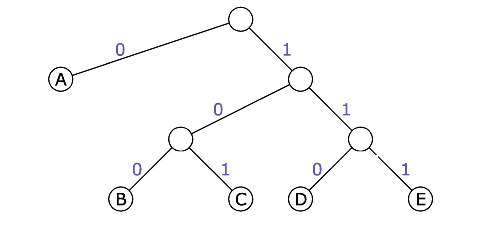
\includegraphics[width=\linewidth]{Huffman-tree.png}
  \caption{Ett exempel på ett Huffman-träd.}
  \label{fig:huffman-tree}
\end{figure}


	\subsubsection{Avkomprimering}
	För att avkomprimera en Huffman-kod behövs samma sannolikhetslista som användes vid komprimeringen av en källa. Förutsatt att denna lista är känd, kan ett Huffman-träd byggas upp på samma vis som vid komprimeringen. Med Huffman-trädet kan man sedan traversera ifrån roten och ner beroende på vilken bit, 0 eller 1, man stöter på i den sekvens som ska avkodas. När man sedan kommer till en lövnod betyder det att en symbol kan avkodas, denna symbol adderas sedan till den resulterande sekvensen. Proceduren startar sedan om ifrån rotnoden och avslutas då det inte längre finns bitar kvar att läsa av i bitsekvensen \cite{huffmancoding2018}.
	
\subsection{LZW-kodning}
LZW-kodning är en metod för att komprimera filer till ett mindre format. Metoden utvecklades av Abraham Lempel, Jacob Ziv, och Terry Welch år 1984. Metoden är en utveckling av den tidigare metoden LZ78 metoden som utvecklades av Abraham Lempel och Jacob Ziv år 1978. Idén med LZW komprimering är att skapa en ordbok för olika symboler och kombinationer av symboler. Med kombinationer av symboler menas symboler som förekommer efter varandra i källan och inte alla möjliga kombinationer av symboler ifrån källan. Nedan beskrivs mer ingående hur komprimering och avkomprimering fungerar i LZW-kodning \cite{lempelzivwelch2018}.
	\subsubsection{Komprimering}
	För att komprimera en given källa med LZW följs dessa steg.
	\begin{enumerate}
	\item Initialisera ordboken så den innehåller alla symboler av längd 1, lämligtvis alla möjliga bytes, 0-255
	\item Hitta den längsta möjliga strängen, W, av symboler i ordboken som matchar den aktuella strängen som avläses.
	\item Addera motsvarande index i ordboken för W till resultatet. 
	\item Addera W plus nästa symbol ifrån källan som avläses till ordboken.
	\item Gå till steg två så länge som det finns kvar symboler att läsa i källan.
	\end{enumerate}
	
	\noindent På detta vis erhålls en sträng med index som för sig motsvarar en eller flera symboler \cite{lempelzivwelch2018}.
 
	\subsubsection{Avkomprimering}
	Avkomprimeringen för en sekvens med LZW-kodning fungerar som följer. Först intialiseras samma ordbok som användes vid komprimeringen, med undantag att man nu mappar index mot en sträng istället för tvärtom. Man läser sedan av ett index ifrån sekvensen och slår upp det indexet i ordlistan, motsvarande symbol/symboler adderas till resultatet. Under tiden byggs ordlistan upp på samma sätt som den byggdes upp under komprimeringen. Det är dock lite annorlunda under avkomprimeringen, när man avläser en symbol, W, vet vi att den sista symbolen i W är ett prefix till nästa symbol, X, som ska vara i ordboken, så vi måste därför vänta tills vi läser av nästa symbol, Y, innan vi kan addera X till ordboken. Avkomprimeringen ligger på så vis ett steg efter med att bygga upp ordboken \cite{lempelzivwelch2018}.
	
%%%%%%%%%%%%%%%%%%%%%%%%%%%%%%%%%%%%%%%%%%%%%%%%%%%%%%%%%%%%%%%%%%%%%%
%%% lorem.tex ends here

%%% Local Variables: 
%%% mode: latex
%%% TeX-master: "demothesis"
%%% End: 
